\documentclass[12pt]{article}
\usepackage{lscape, xcolor}
\usepackage{verbatim}
\usepackage{amsmath,amsthm,amssymb}
\usepackage{colonequals,color,multirow}
\usepackage{enumerate}
\usepackage[sc]{mathpazo} % Use the Palatino font
\usepackage[T1]{fontenc} % Use 8-bit encoding that has 256 glyphs
\usepackage{times}	
% \usepackage{apacite}
\usepackage[authoryear]{natbib}
\usepackage[demo]{graphicx}
\usepackage{subcaption}
\usepackage{lscape, xcolor}
\usepackage{verbatim}
\usepackage{amsmath,amsthm,amssymb}
\usepackage[sc]{mathpazo} % Use the Palatino font
\usepackage[T1]{fontenc} % Use 8-bit encoding that has 256 glyphs
\usepackage{times}	
\usepackage{booktabs}
\usepackage{ caption, float}
\usepackage{enumitem}
\usepackage[left=1in, right=1in, top=1in, bottom=1in]{geometry}
\usepackage{blindtext}
\usepackage{titlesec}
\usepackage{array}
\usepackage{graphicx}
%\graphicspath{/home/evo/4m_final_project}
\setcounter{secnumdepth}{4}
\usepackage{caption} % For subfigures with captions
\usepackage{subcaption} % For subfigures with captions
\captionsetup[subfigure]{labelformat=empty} % Removes the (a), (b) labels
\usepackage{hyperref}
\usepackage[authoryear]{natbib}
\usepackage{setspace}
%\onehalfspacing % Sets one-and-a-half line spacing globally
\titleformat{\paragraph}
{\normalfont\normalsize\bfseries}{\theparagraph}{1em}{}
\titlespacing*{\paragraph}
{0pt}{3.25ex plus 1ex minus .2ex}{1.5ex plus .2ex}
\renewcommand{\baselinestretch}{1.5}% Line spacing - Palatino needs more space 
\vspace{\baselineskip}
\linespread{1.5}
\setlength{\parskip}{0.5em} % Adjust spacing to 0.5em (smaller than default)


\begin{document}

\title{STATS 4M03: Multivariate Analysis\\ Final Project \\ Diabetes Dataset }

\author{Submitted to\\ Dr. Eman M.S. Alamer 
\\Department of Mathematics and Statistics
\\McMaster University\\Hamiltion, Ontario, Canada L8S 4K1}
\date {November 22, 2024}


\maketitle

 \centerline{Reported by}
 \centerline{Safi Khan (400402095)}
 \centerline{Tonu Xu (400370837)}
 \centerline{Xinyi Chen (400326045)}
 \centerline{Rayyan Kazim (400406943)}
 \centerline{Zesen Chen (400326984)}


\newpage
%\thispagestyle{fancy} % All pages have headers and footers
\section{Introduction}
\subsection{Abstract}



\begin{indent} 
\onehalfspacing	
	
The study of diabetes is vital in understanding the progression of the disease and identifying key predictors. Throughout this paper, we perform data analysis on the \href{https://www.kaggle.com/datasets/hasibur013/diabetes-dataset}{diabetes dataset}, primarily focusing on leveraging various supervised learning analysis methods that we learned in STATS 4M03$\backslash$6M03: Multivariate Analysis. By using a variety of methods, our goal is to predict the onset of diabetes from detailed medical diagnostic measurements based on several contributing health factors --- to uncover patterns and relationships between various clinical and lifestyle factors. Through this analysis, we hope to emphasize actionable insights for clinical decision-making and provide preventive strategies. 
\end{indent}

\subsection{The Data}

\begin{indent}
\onehalfspacing	
	
We will study the \href{https://www.kaggle.com/datasets/hasibur013/diabetes-dataset}{diabetes dataset} from \cite{Kaggles}, which contains 768 rows x 9 columns. Each column represents various health diagnostic metrics for predicting diabetes and each row corresponds to a unique patient record. Table~\ref{tab:DibetesTab} showcases a description for each of the columns in the dataset, and we will be using R as our main computing software \citep{Rlang}.
\end{indent}


\begin{table}[h!]
	\centering
	\resizebox{=\textwidth}{!}{ % Resize to fit the width of the page
	\begin{tabular}{|c|c|}
		\hline
		\textbf{Column} & \textbf{Description Of Column} \\ \hline
		Pregnancies & Integer: Number of times the patient has been pregnant. \\ \hline
		Glucose & Integer: Plasma glucose concentration (mg/dL) after a 2-hour oral glucose tolerance test. \\ \hline
		BloodPressure & Integer: Diastolic blood pressure (mm Hg). \\ \hline
		SkinThickness & Integer: Triceps skinfold thickness (mm). \\ \hline
		Insulin & Integer: 2-hour serum insulin (mu U/ml). \\ \hline
		BMI  & Float: Body mass index, defined as weight in kg/(height in m)\^2. \\ \hline
		DiabetesPedigreeFunction & Float: A score indicating genetic predisposition to diabetes based on family history. \\ \hline
		Age & Integer: Age of the patient (in years). \\ \hline
		Outcome & Binary: Target variable where 1 indicates diabetes, and 0 indicates no diabetes. \\ 
		\hline
	\end{tabular}
}
	\caption{Column Descriptions of the Diabetes Dataset}
	\label{tab:DibetesTab}
\end{table}


\subsubsection{Exploratory Data Analysis (EDA)}

\begin{indent}
\onehalfspacing	
	
The true label of this dataset is Outcome, whereas the other variables are considered the predictors. Since our dataset is not that large, we determined that we should use all of the predictors as they all show reasonably high correlation with each other. 

Figure~\ref{fig:outcomeplot} illustrates that there are a lot more individuals in the dataset who do not have diabetes. Figure~\ref{fig:ageplot} showcases that the ages listed in this dataset follow a right-skewed distribution, where majority of the individuals are aged 20-30.

Figure~\ref{fig:corplot} illustrates the relatively high correlation between SkinThickness, BMI, and Insulin. We also note that Glucose is reasonably correlated with Insulin, BMI, and Age. Furthermore, Age is highly correlated with Pregnancies.

We cannot apply factor analysis on our dataset as it is not normally distributed. This can be confirmed by the Shapiro-Wilk test and normal QQ plot in Figure~\ref{fig:qqplot} \citep{Rlang}.
\end{indent}

 \begin{figure}[h!]
 	\centering
 	% First figure
 	\begin{minipage}{0.48\textwidth}
 		\fbox{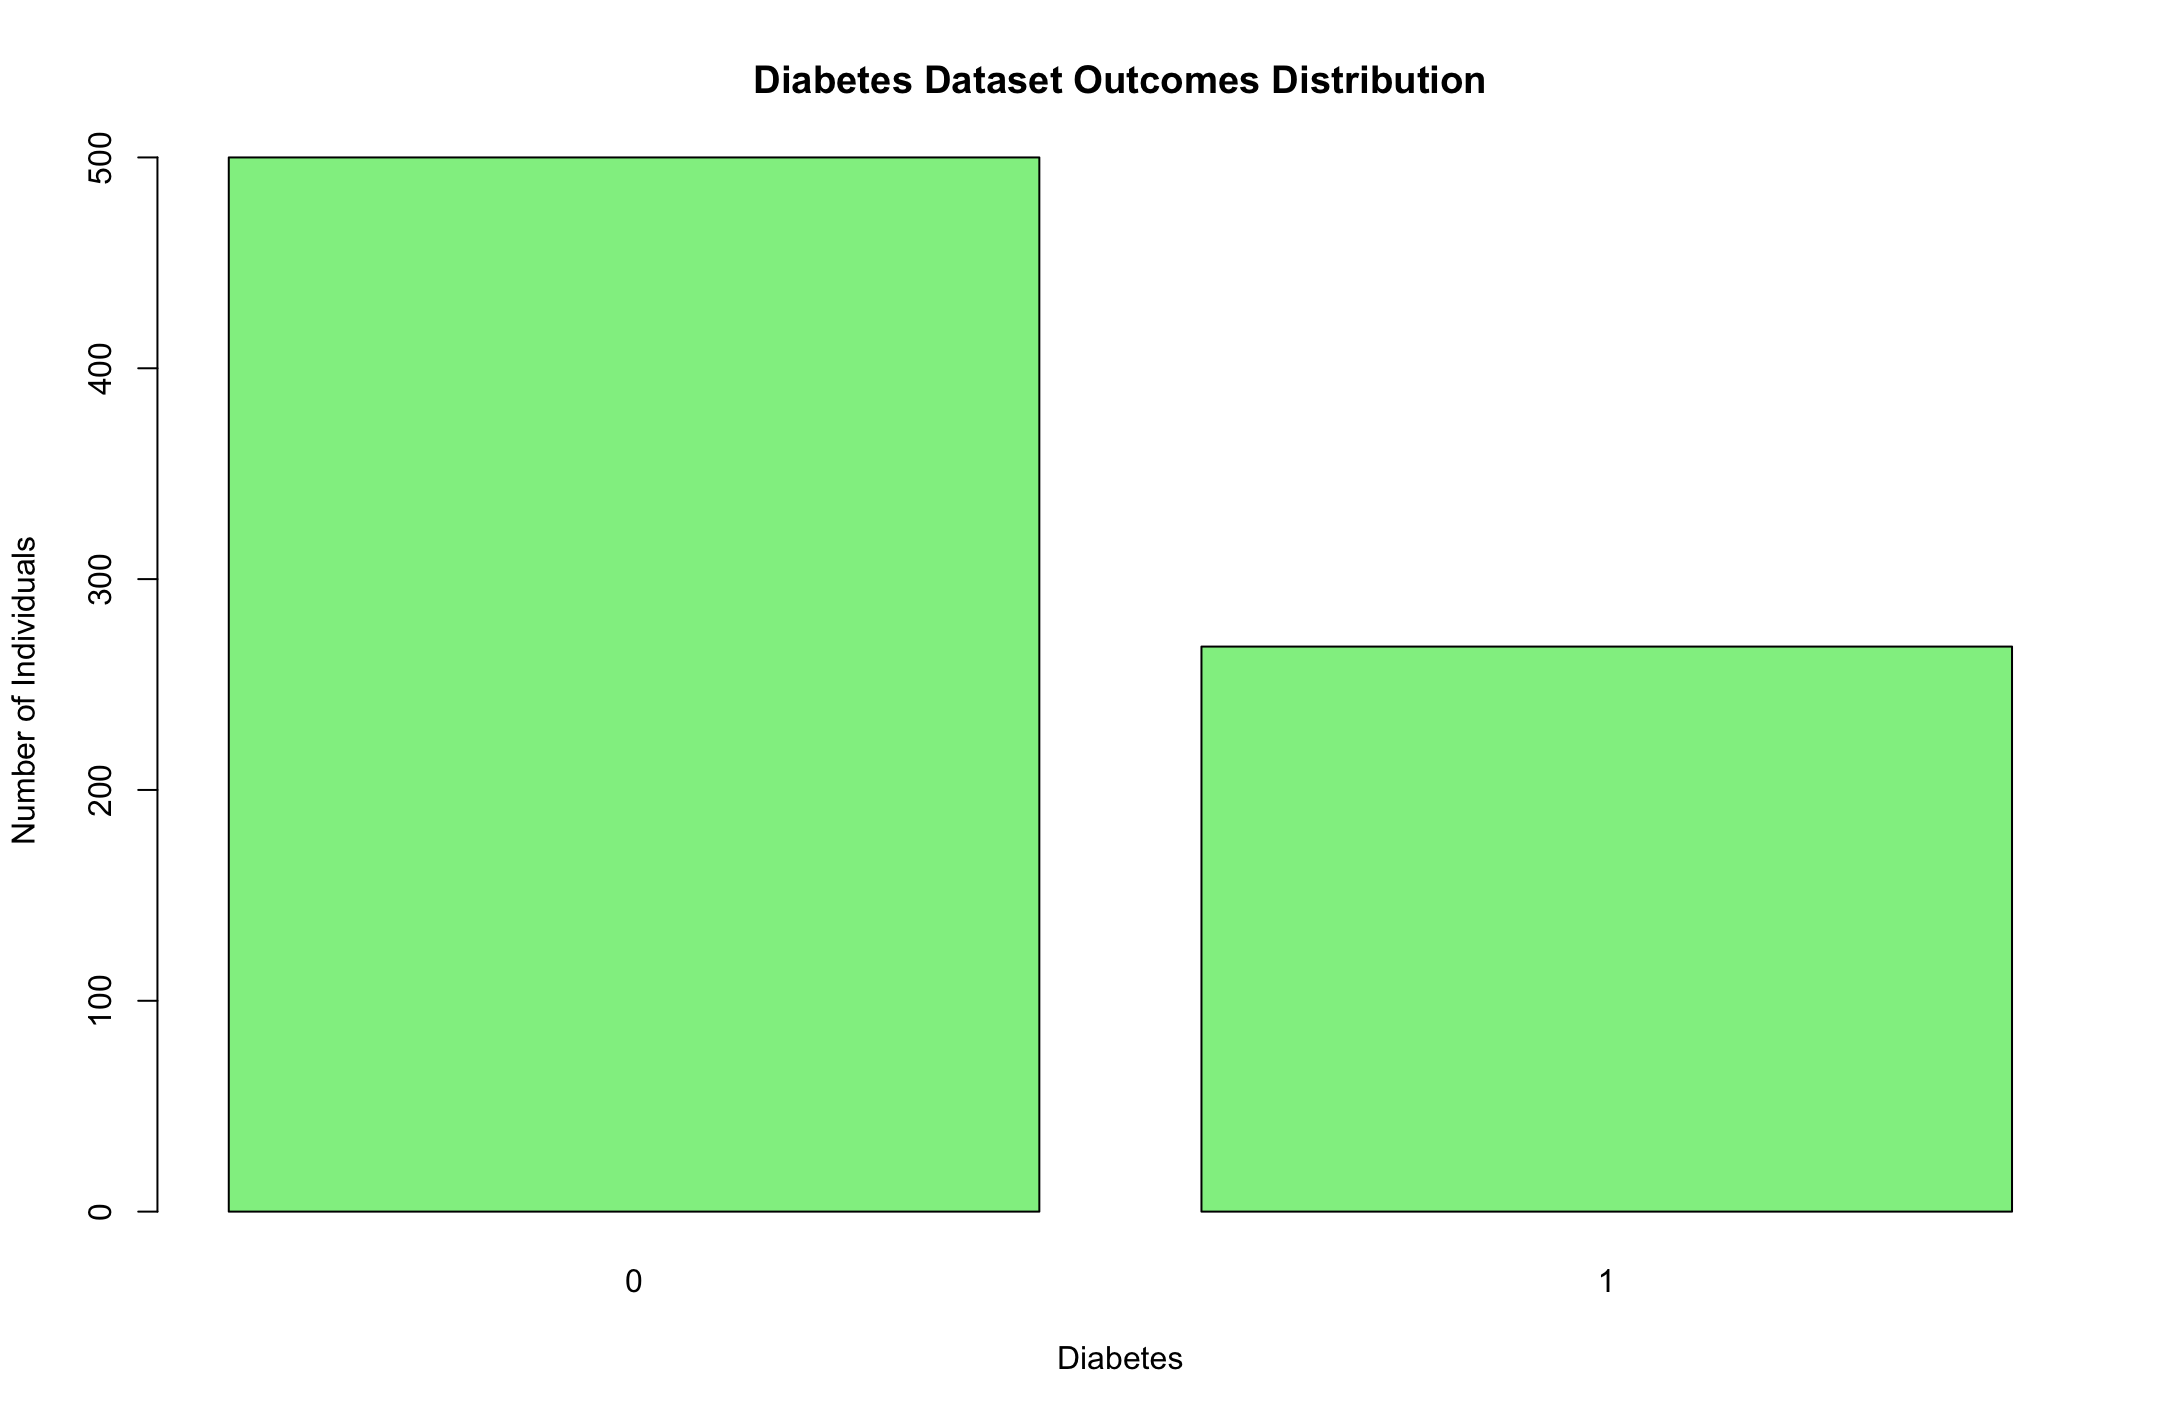
\includegraphics[width=\textwidth]{outcomes.png}} 
 		\caption{Distribution of Outcomes} 
 		\label{fig:outcomeplot}
 	\end{minipage}
 	\hfill % Horizontal space between figures
 	% Second figure
 	\centering
 	\begin{minipage}{0.48\textwidth}
 		\centering
 		\fbox{{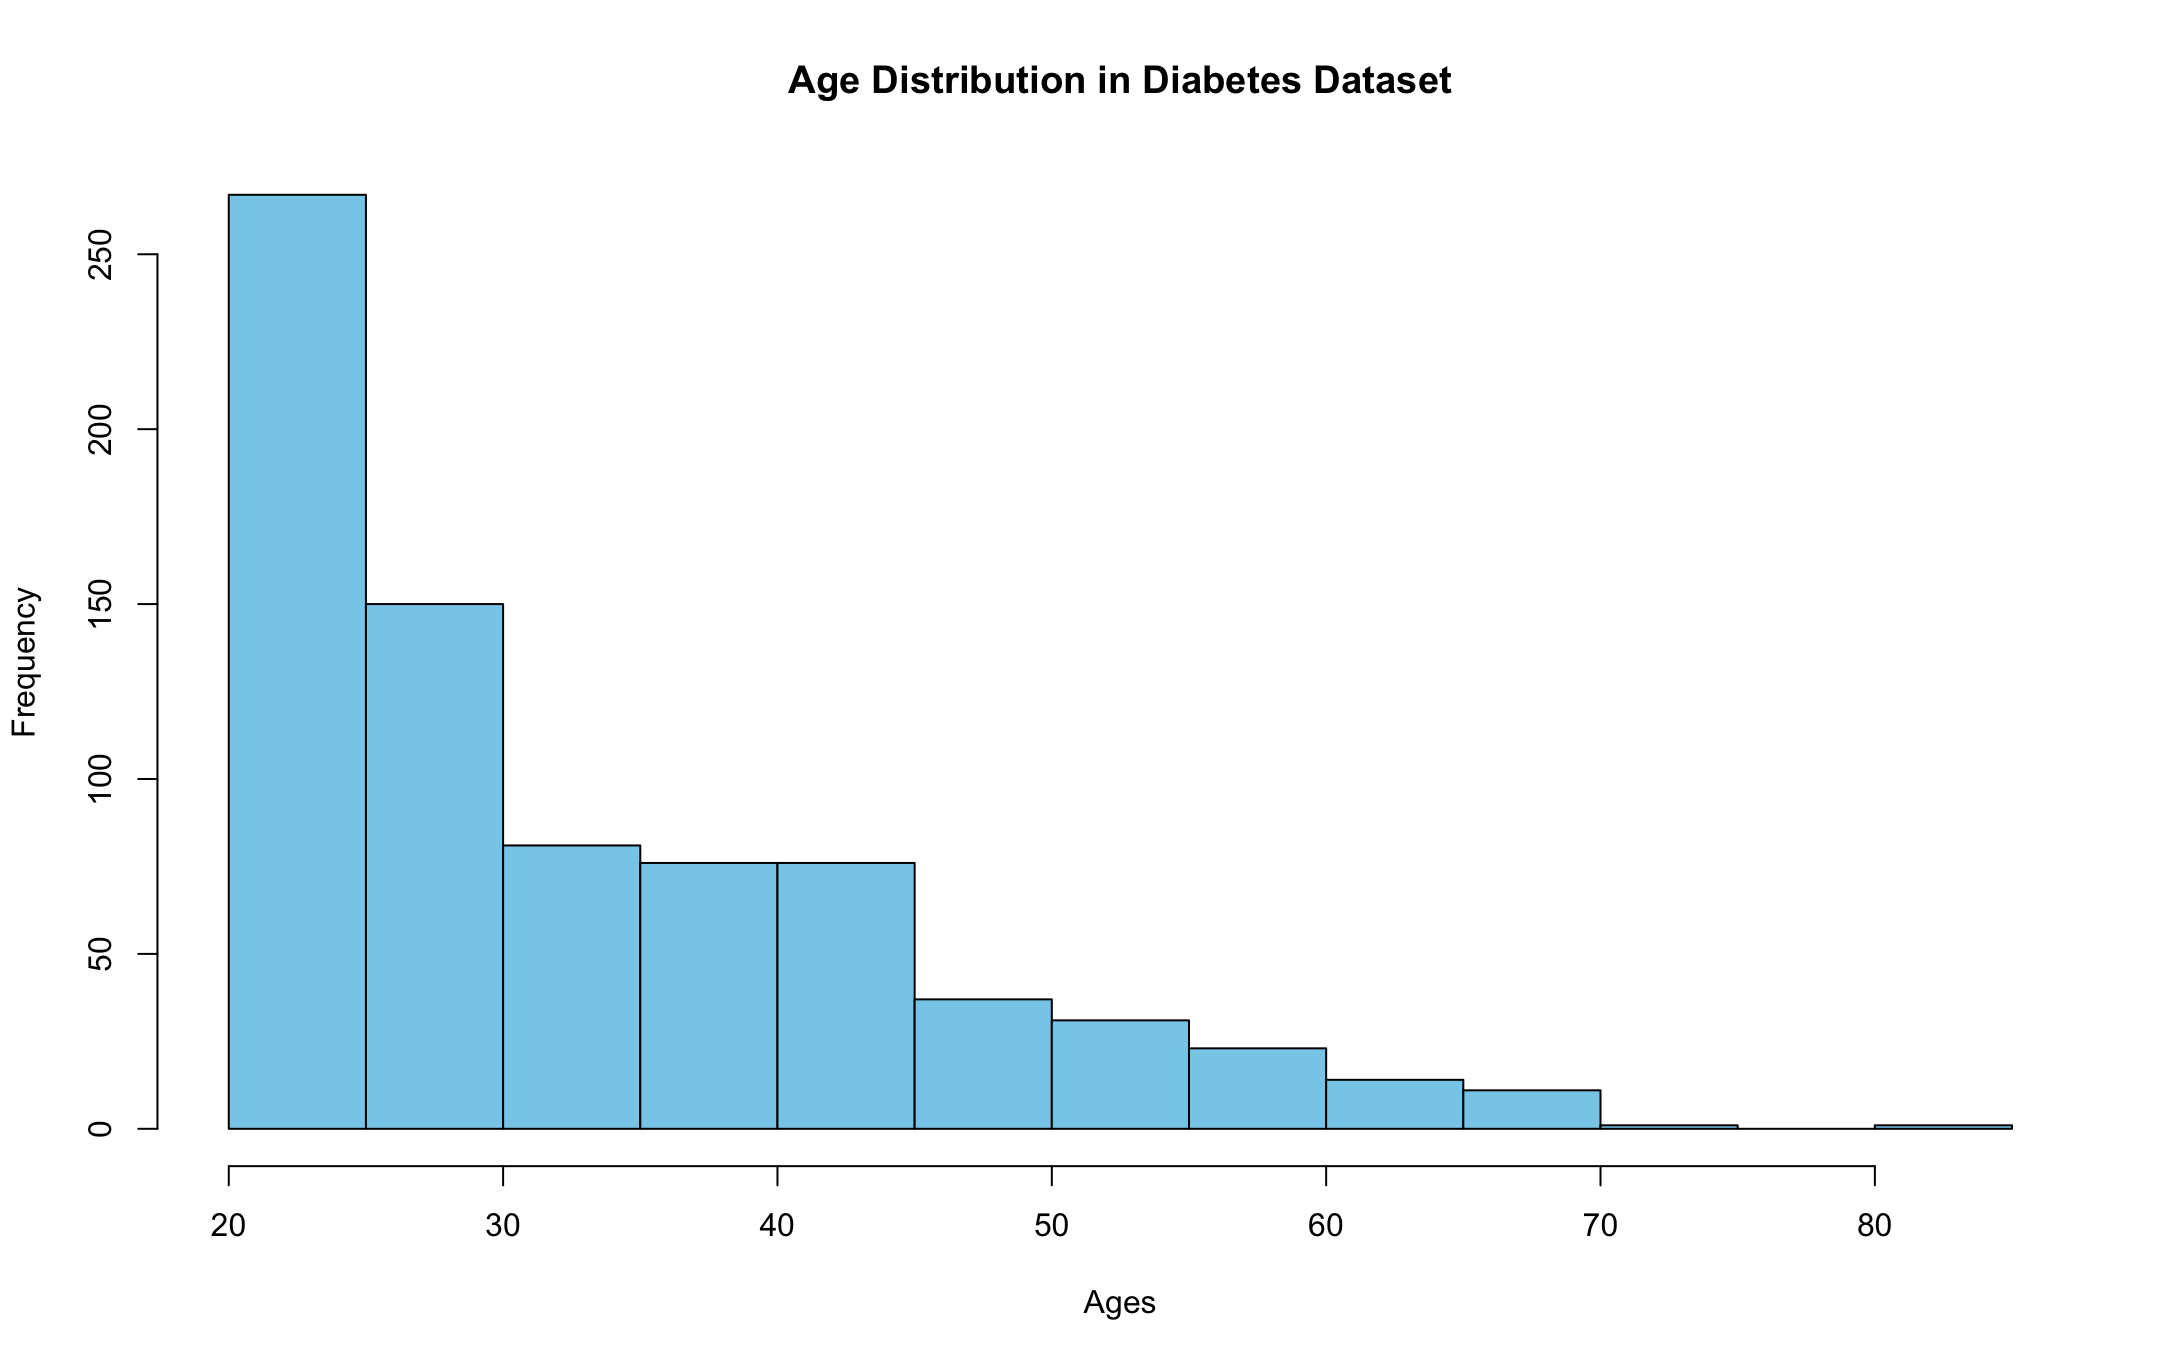
\includegraphics[width=\textwidth]{ages.png}}}
 		\caption{Age Distribution of the Dataset} 
 		\label{fig:ageplot}
 	\end{minipage}
 \end{figure}

 \begin{figure}[h!]
 	\centering
 	% First figure
 	\begin{minipage}{0.48\textwidth}
 		\fbox{{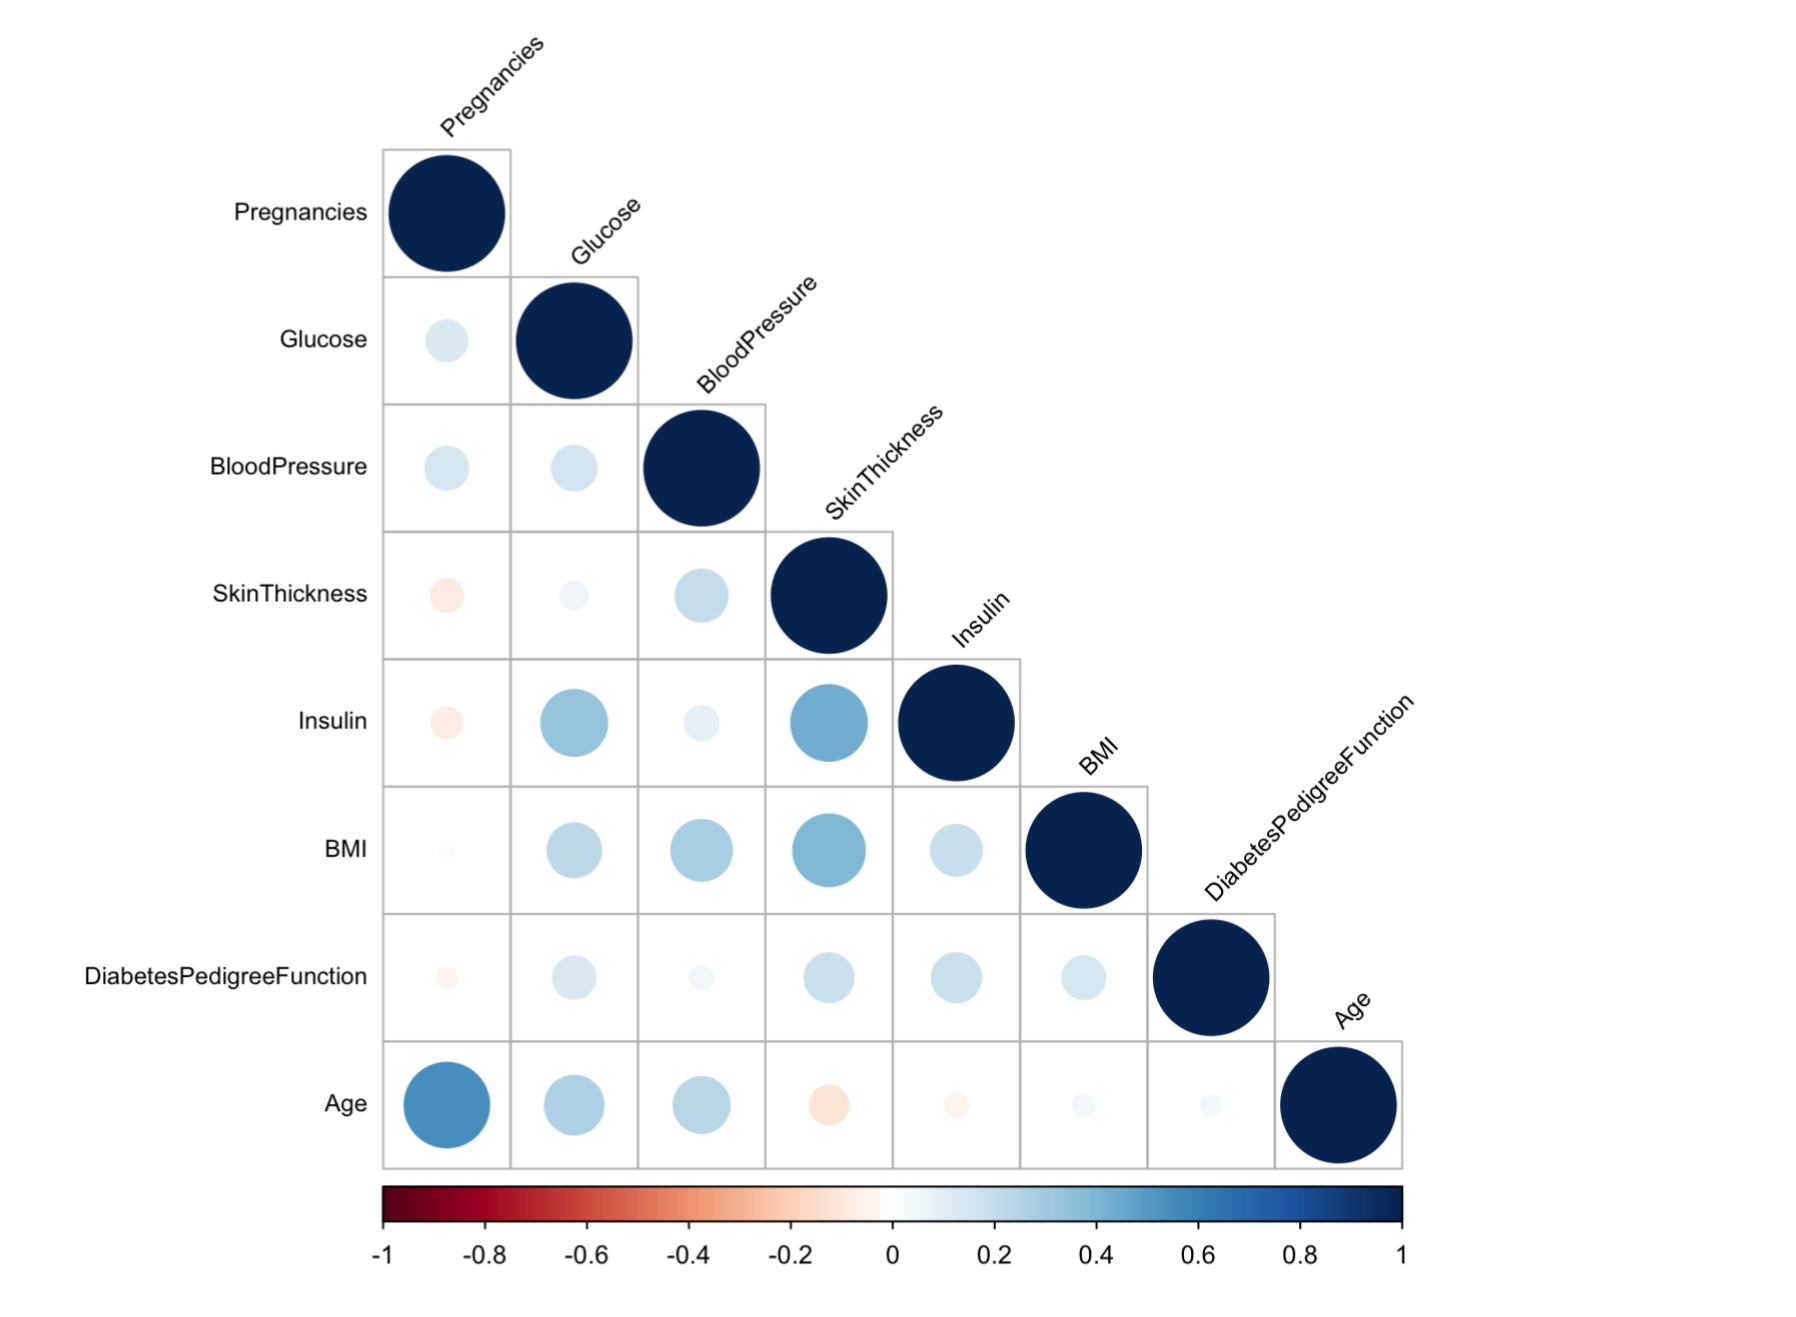
\includegraphics[width=\textwidth]{correlations2.png}}}
 		\caption{Correlation of Variables} 
 		\label{fig:corplot}
 	\end{minipage}
 	\hfill % Horizontal space between figures
 	% Second figure
 	\centering
 	\begin{minipage}{0.48\textwidth}
 		\centering
 		\fbox{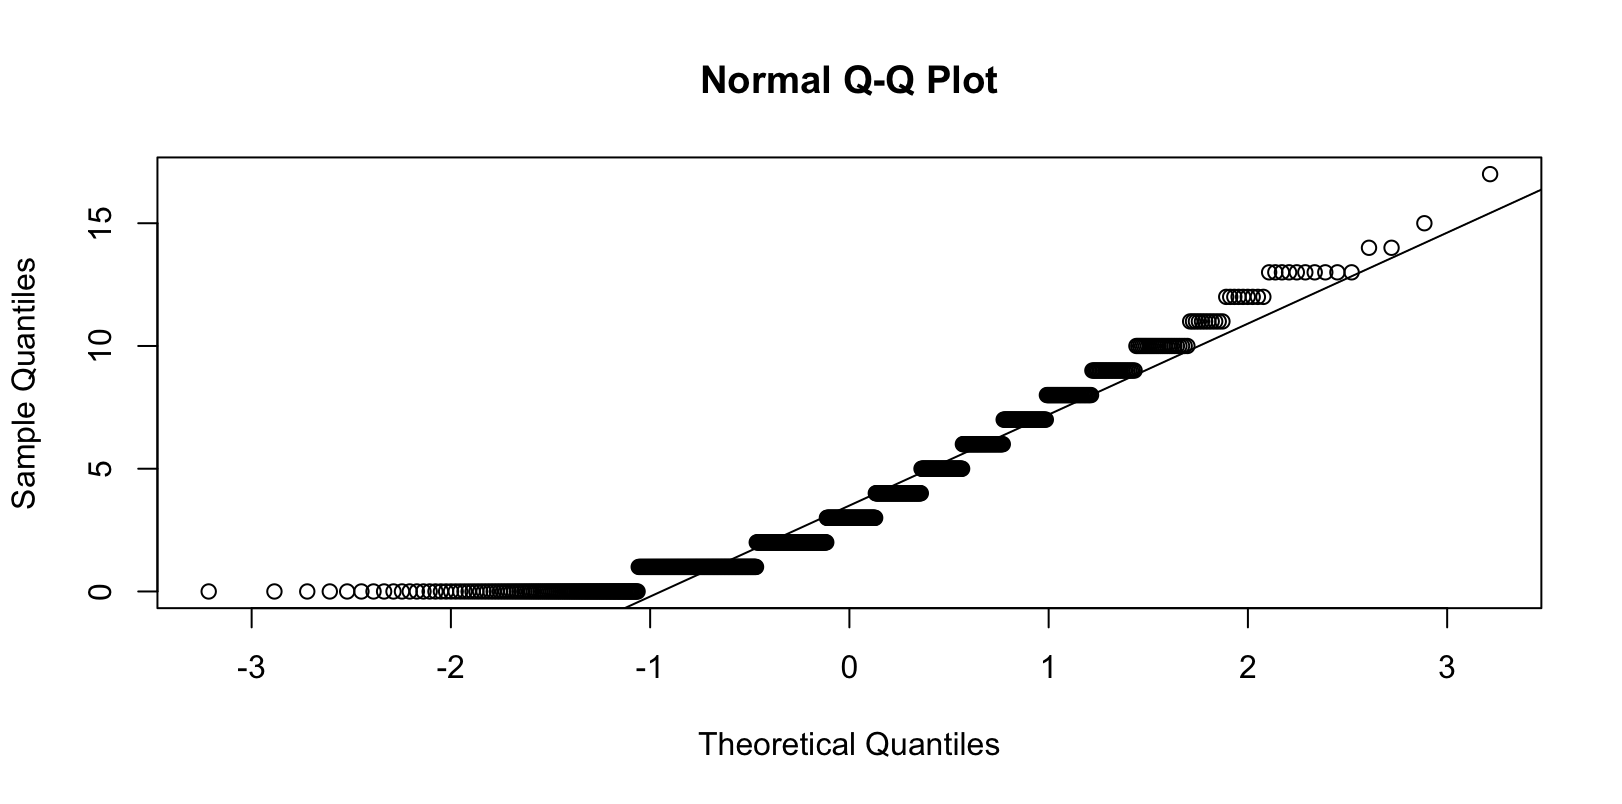
\includegraphics[width=\textwidth]{normal.png}} 
 		\caption{Normal QQ-Plot} 
 		\label{fig:qqplot}
 	\end{minipage}
 \end{figure}
		
\subsubsection{Data Preparation} 

\begin{indent}
\onehalfspacing
	
We prepared the data by scaling all the columns in the dataset except for column nine which is the response variable, Outcome, the true label of this dataset. We will split the data as follows: 75\% for training to allow each of the models to learn effectively, and 25\% will be reserved for testing to evaluate each of the models' performance on unseen data. Additionally, we will retain all variables in the model due to the relatively moderate to high association between each of the predictor variables.


\end{indent}

\section{Methodology}
 
\subsection{k-Nearest Neighbours}

\indent
\onehalfspacing

We executed the k-Nearest Neighbours algorithm (k-NN), a non-parametric, supervised learning classifier that uses proximity to make classifications about the grouping of a dataset. \citep{peterson2009k,7724478}. Specifically, the algorithm takes an unlabelled observation and assigns it to the class that has the most labelled observations within its neighbourhood. \citep{Lecture14}. Additionally, we note that the optimal k-value will result in the best classification rate, based on the labelled points that are being treated as unlabelled by the algorithm \citep{Lecture14}.

 \subsection{Random Forest Classifiers}
 
\indent
\onehalfspacing

We also utilized the Random Forest Classifiers algorithm on our dataset \citep{zhou2012ensemble}. Random Forest is a bootstrapping sampling method that combines the results of multiple decision trees to draw on a conclusion \citep{7724478}. The algorithm is an extension of the bagging algorithm which creates uncorrelated decision trees. For each tree, a random sample of $\mathcal{M}$ predictors is taken at each decision tree split for each of the $M$ trees, with the goal of improved predictive model accuracy \citep{Lecture16}.

\subsection{Binary Logistic Regression}

\begin{indent}
\onehalfspacing
	
We performed binary logistic regression on our dataset to explore the relationship and significance between our predictor variables and the binary response variable, Outcome \citep{faraway2016extending}. We identify the most significant predictors using backward elimination, a step-wise technique employed in regression to minimize the risk of overfitting. This means that predictors whose $p$-value is greater than $\alpha = 0.05$ level of significance will be removed and we will run the algorithm again, repeating this process until we end up with only statistically significant predictors in our model.
\end{indent}

\subsection{Boosting}

\begin{indent}
\onehalfspacing
	
Boosting is one of the ensemble methods which combines multiple weak learners, typically decision trees, to create a strong predictive model \citep{chen2015xgboost,friedman2001greedy}. For this analysis, we used XGBoost (Extreme Gradient Boosting), which is efficient and well optimized for large datasets, to predict the presence of diabetes based on our predictor variables. 
\end{indent}

\textbf{Model Parameters}; Learning rate (\texttt{eta}): 0.1, Maximum tree depth (\texttt{max\_depth}): 6, Evaluation metric: Area Under the ROC Curve (AUC), and Number of boosting rounds (\texttt{nrounds}): 100

\section{Discussion}

\subsection{k-Nearest Neighbours}

\indent
\onehalfspacing

After tuning the algorithm using a $5$-fold cross-validation to get the optimal parameters for the k-nearest neighbours algorithm (k-NN), we found that the best value for $k$ is $3$, which can be observed in Figure~\ref{fig:KNNPlot}. This result indicates that if $2$ out of the $k = 3$ neighbours have a positive response for diabetes, the individual will be assigned a positive response for diabetes, i.e. Outcome = 1. Conversely, if $2$ out of the $k = 3$ neighbours have a non-positive response for diabetes, the individual will be assigned a non-positive response, i.e. Outcome = 0. After inputting $k=3$ and running the k-NN algorithm, we found that the MCR given by k-NN classification is $0.2916667$, i.e. $\sim71\%$ of the individuals predicted to have a positive or non-positive response for diabetes were correctly classified.

\begin{figure}[h!]
	\centering
	\fbox{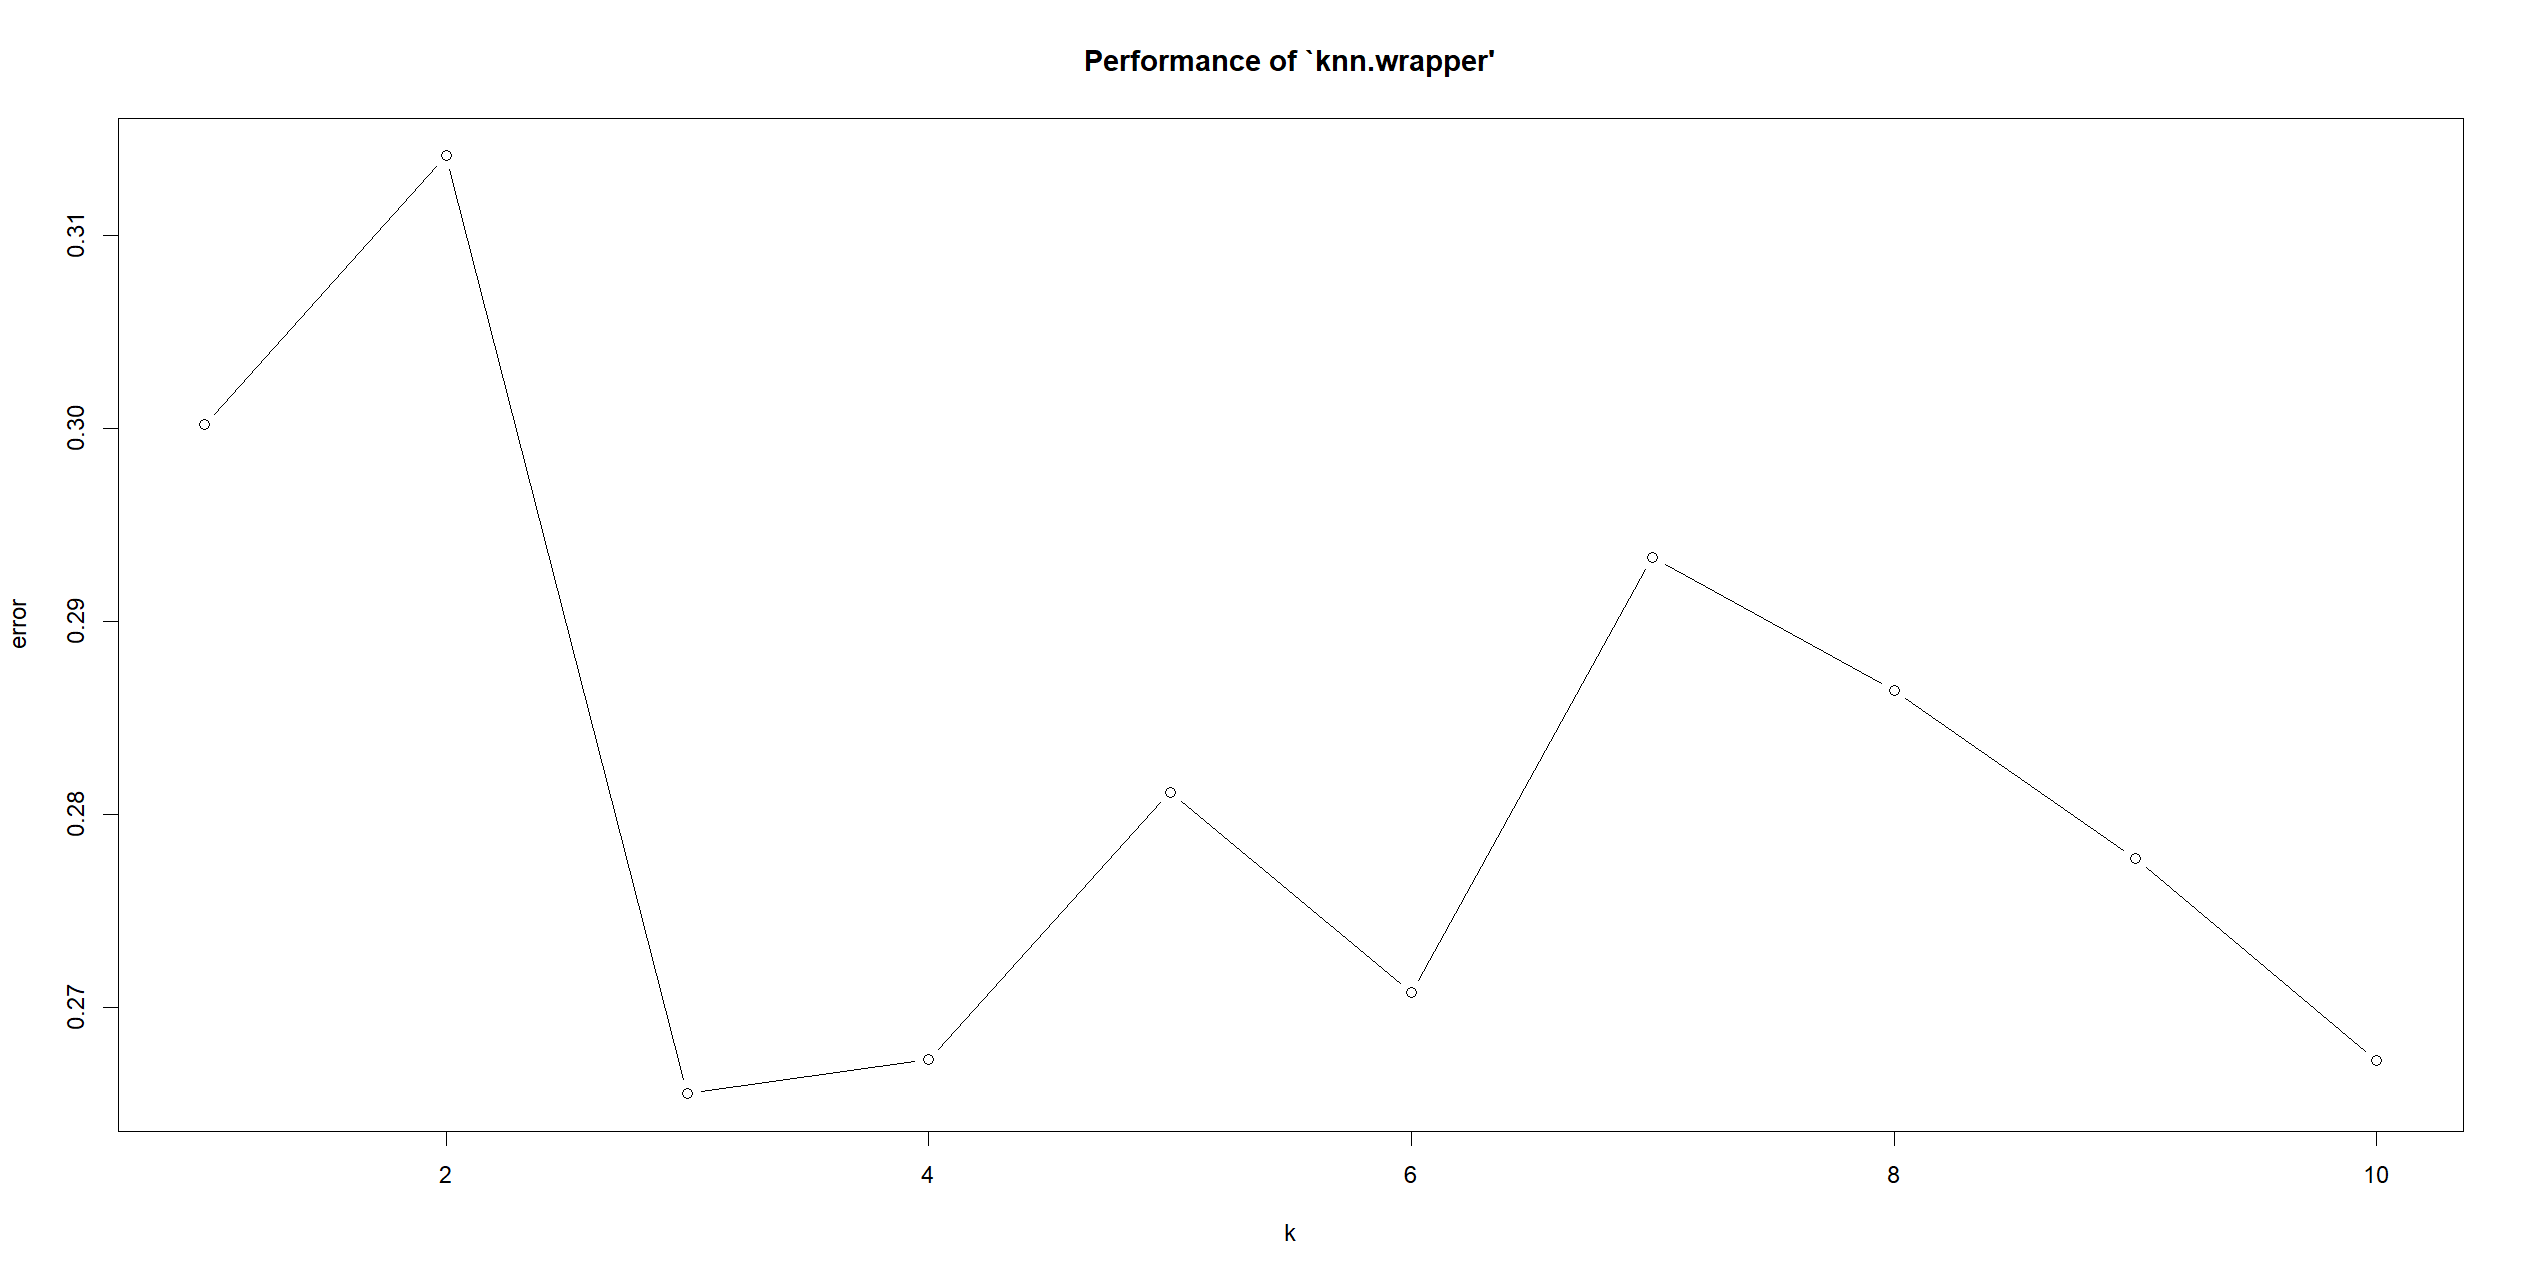
\includegraphics[width=0.80\textwidth]{knnplot.png}} 
	\caption{Output Plot From k-NN Classification} 
	\label{fig:KNNPlot}
\end{figure}

\subsection{Random Forest Classifiers}

\begin{indent}
	\onehalfspacing
	
After tuning the algorithm using a $5$-fold cross-validation to get the optimal parameters for the random forest algorithm, we found that the best value for $\mathcal{M}$ is $4$ and the best value of $M$ is $200$. 
	
After inputting $\mathcal{M}$ = $4$ and $M$ = $200$ into the random forest algorithm, we found that the MCR given by random forest classification is $0.28125$, i.e. $\sim72\%$ of the individuals predicted to have a positive or non-positive response for diabetes were correctly classified. Consequently, Figure~\ref{fig:RFPlot} highlights that Glucose and BMI are the most important predictor variables, and excluding them from the model will lead to worse accuracy in predicting the Outcome. Conversely, SkinThickness and BloodPressure are the least important predictors and excluding them will not greatly affect the accuracy of the model.
\end{indent}

\begin{figure}[h!]
	\centering
	% First figure
	\fbox{{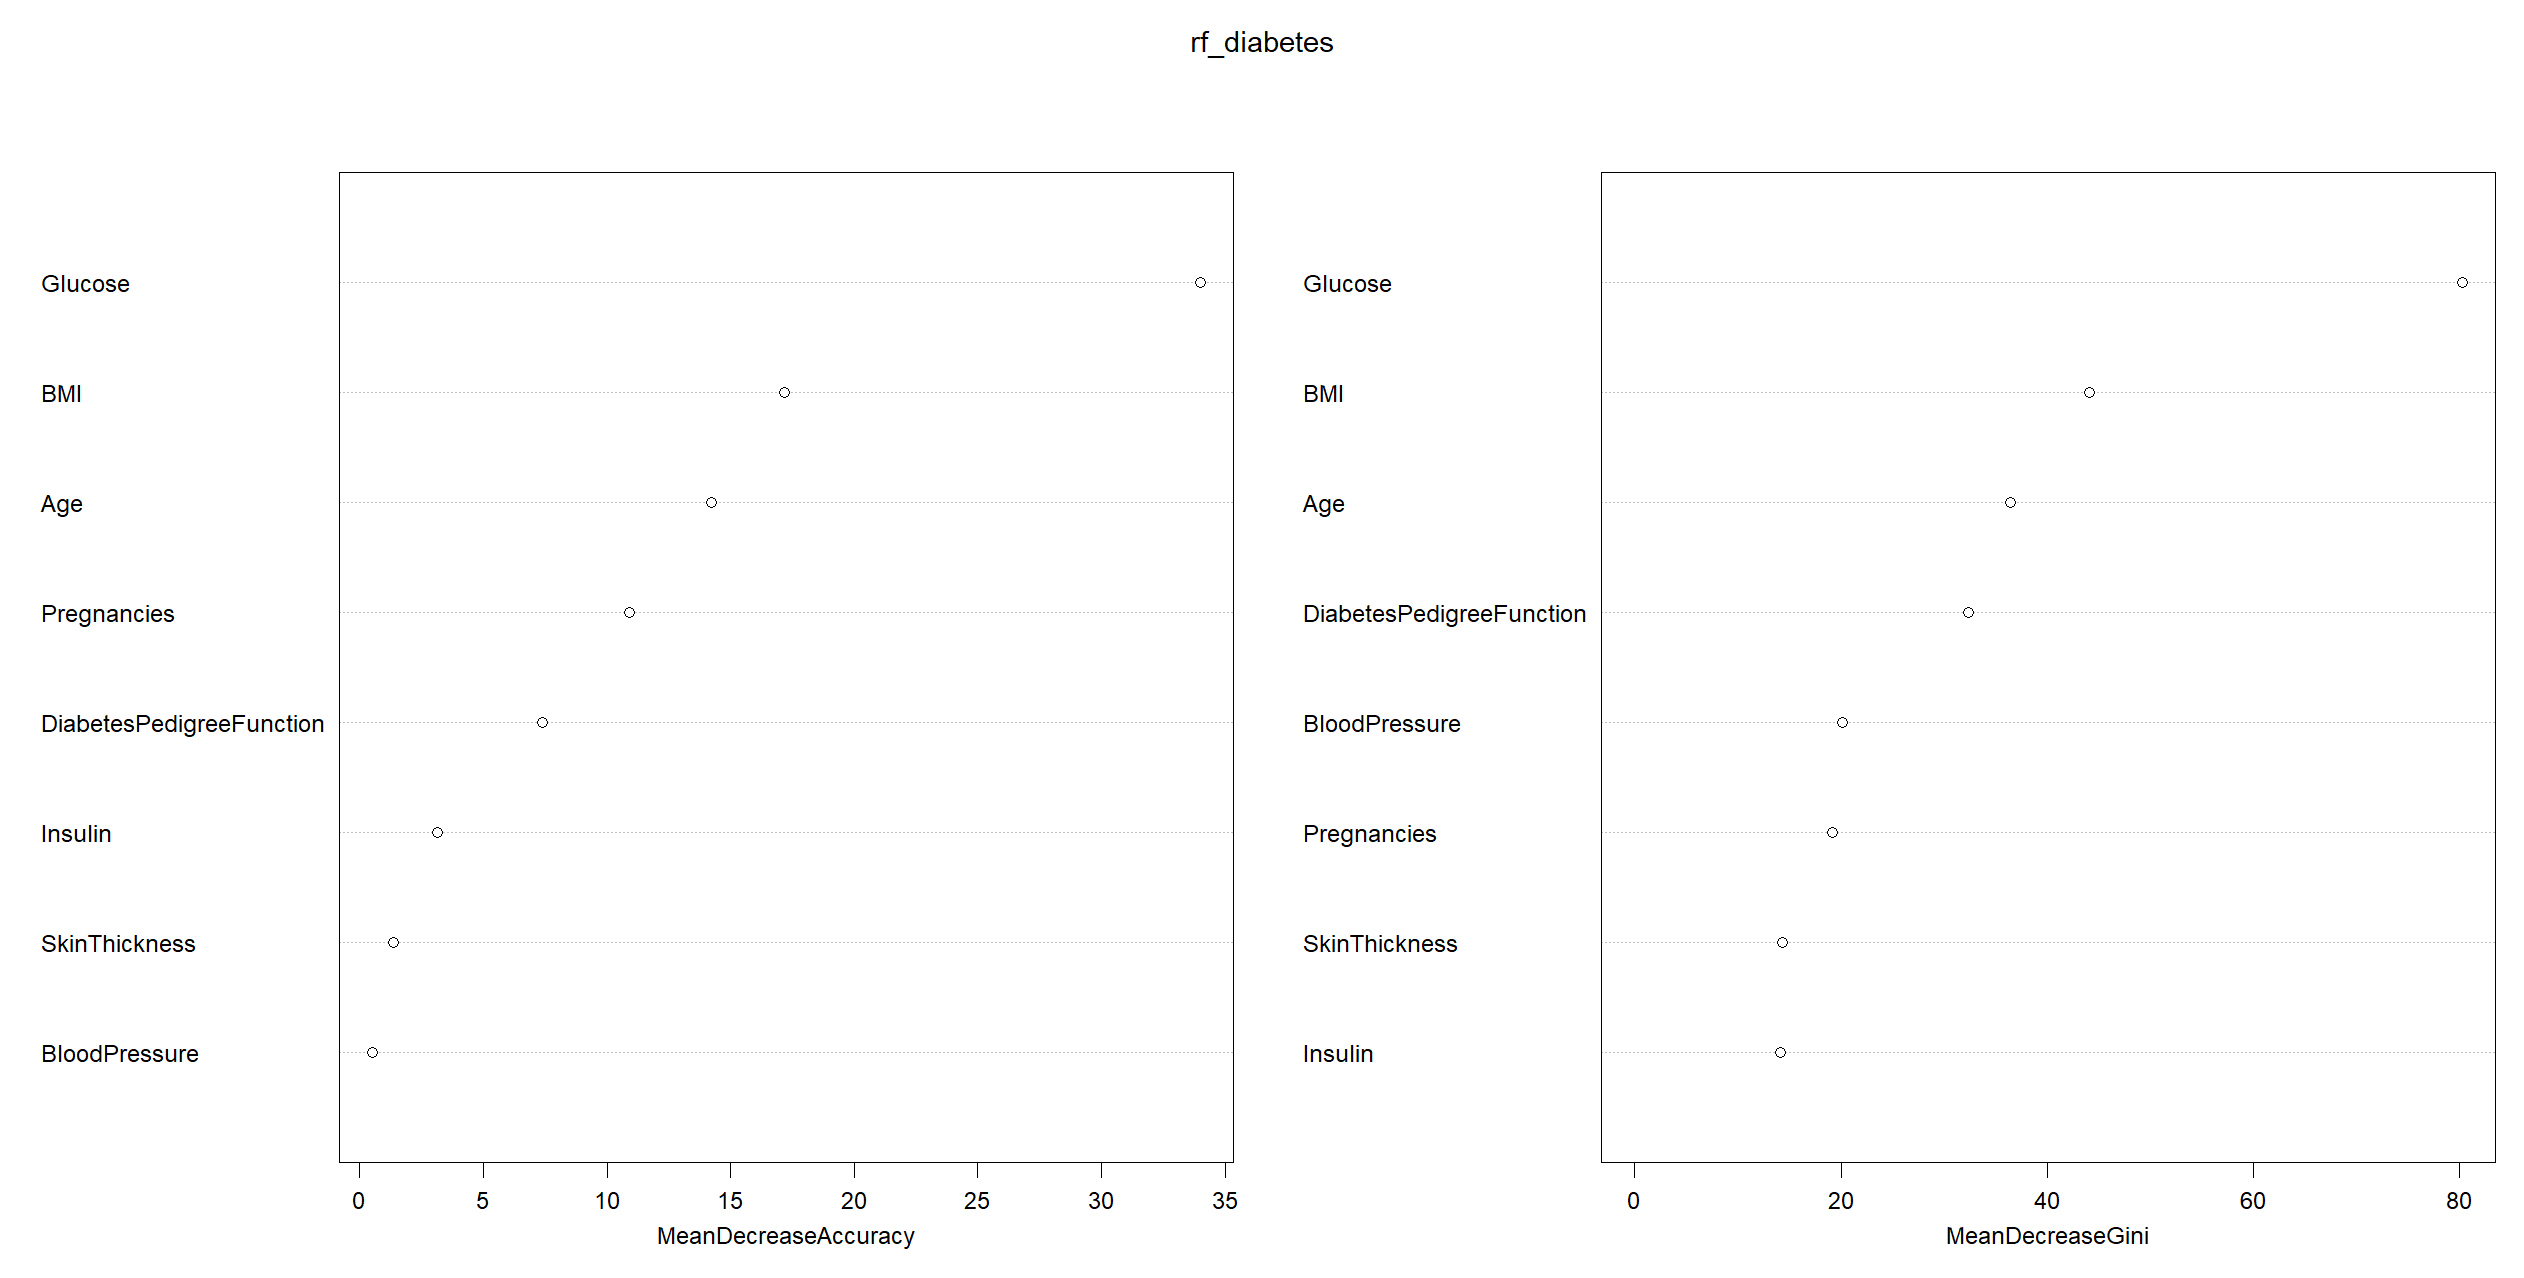
\includegraphics[width=0.80\textwidth]{MeanDecreaseAccuracyPlotForRandomForest.png}}}
	\caption{MeanDecreaseAccuracy {\&}\ MeanDecreaseGini Plot from Random Forest} 
	\label{fig:RFPlot}
\end{figure}

\subsection{Binary Logistic Regression}

\begin{table}[h!]
	\centering
	\resizebox{=\textwidth}{!}{
		\begin{tabular}{|l|l|l|l|l|}
			\hline
			\textbf{Coefficients} & \textbf{Estimate} & \textbf{Std. Error} & \textbf{Z-Value} & \textbf{Pr(>|Z|)} \\ \hline
			(Intercept) & -0.863576 & 0.111504 & -7.745 & 9.57E-15 \\ \hline
			Pregnancies & 0.411598 & 0.128257 & 3.209 & 1.33E-03 \\ \hline
			Glucose & 1.003291 & 0.133428 & 7.519 & 5.51E-14 \\ \hline
			BloodPressure & -0.15522 & 0.122145 & -1.271 & 0.2038 \\ \hline
			SkinThickness & -0.008376 & 0.123519 & -0.068 & 0.94594 \\ \hline
			Insulin & -0.160385 & 0.120504 & -1.331 & 1.83E-01 \\ \hline
			BMI & 0.699525 & 0.135793 & 5.151 & 2.59E-07 \\ \hline
			DiabetesPedigreeFunction & 0.295516 & 0.114215 & 2.587 & 0.00967 \\ \hline
			Age & 0.212147 & 0.127142 & 1.669 & 0.0952 \\ \hline
		\end{tabular}
	}
	\caption{Binary Logistic Regression Full Model Output}
	\label{tab:BinLogReg}
\end{table}

\indent 
\onehalfspacing

From (Table~\ref{tab:BinLogReg}), we see that the coefficients for BloodPressure, SkinThickness, Insulin, and Age have high p-values, indicating that at $\alpha = 0.05$ level of significance, they are not significant in predicting the Outcome. At this step, the MCR given by the full binary logistic regression model is 0.3697917.

\begin{table}[h!]
	\centering
	\resizebox{=\textwidth}{!}{
		\begin{tabular}{|l|l|l|l|l||l|}
			\hline
			Coefficients: & Estimate & Std. Error & z value & Pr(>|z|) & Odds Ratio \\ \hline
			(Intercept)   & -8.118918 & 0.730397 & -11.116 & <2e-16 & --- \\ \hline
			Pregnancies   & 0.154186  & 0.032151 & 4.796   & 1.62E-06 & 1.167 \\ \hline
			Glucose       & 0.030679  & 0.003781 & 8.113   & 4.92e-16 & 1.031 \\ \hline
			BMI           & 0.080086  & 0.016048 & 4.990   & 6.03e-07 & 1.083 \\ \hline
			DiabetesPedigreeFunction & 0.863621 & 0.336274 & 2.568 & 0.0102 & 2.372 \\
			\hline
		\end{tabular}
	}
	\caption{Binary Logistic Regression Reduced Model Output with Odds Ratio}
	\label{tab:BinLogRegA}
\end{table}

Table~\ref{tab:BinLogRegA} showcases the output from the reduced Binary Logistic Regression Model. We observe that the $p$-values for all the predictors in the model are less than $\alpha = 0.05$, indicating that they're statistically significant in predicting the response variable, Outcome. Furthermore, the MCR has decreased to $0.2395833$, i.e. $\sim76\%$ of the individuals predicted to have a positive or non-positive response for diabetes were correctly classified, showcasing an improvement in the performance of the model. 

Furthermore, Table~\ref{tab:BinLogRegA} highlights the Odds Ratios (OR) for the predictors in the model. Note that each OR is greater than 1, suggesting increased likelihoods of the presence of diabetes with respect to the predictors. Specifically, the OR for Pregnancies is 1.167, indicating that females with a history of pregnancies are 1.167 times more likely to have diabetes than those without. Most significantly, the OR for DiabetesPedigreeFunction is 2.372, meaning that females who indicate a genetic predisposition to diabetes based on family history are 2.372 times more likely to develop diabetes than those without a genetic predisposition. The OR for the other predictors can be interpreted similarly. 

\subsection{Boosting}

\indent
\onehalfspacing

Boosting achieved an accuracy of 73.44\%, with an AUC of 0.802. The AUC is the area under the ROC curve (Figure~\ref{fig:roc}). The ROC Curve is a plot of the model’s Sensitivity (True Positive Rate) against the Specificity (True Negative Rate), illustrating how well the model distinguishes between classes across all possible thresholds \citep{fawcett2006introduction}. The AUC is the area under the ROC curve, summarizing the model's overall ability to discriminate between positive and negative classes. An AUC of 0.5 represents random guessing, while an AUC closer to 1.0 indicates excellent performance \citep{pROC,fawcett2006introduction}.

\begin{figure}[h!]
	\centering
	\fbox{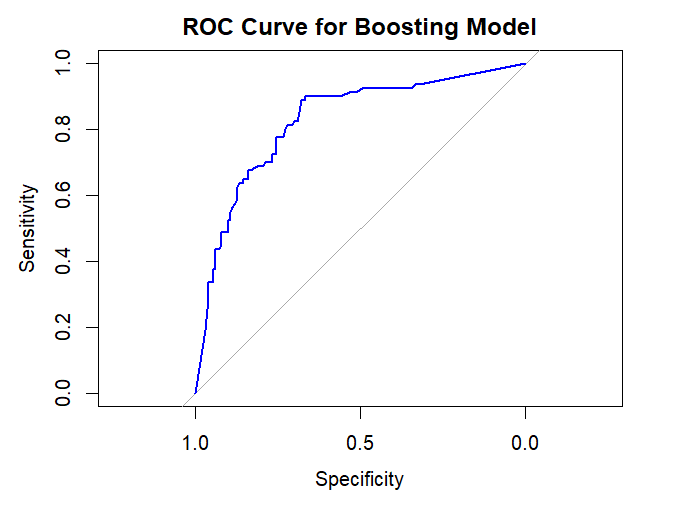
\includegraphics[width=0.80\textwidth]{"C:/Users/msafi/OneDrive/Documents/GitHub/4m_final_project/G2.png"}}
	\caption{ROC Curve for Boosting Model}
	\label{fig:roc}
\end{figure}

\begin{figure}[h!]
	\centering
 	\fbox{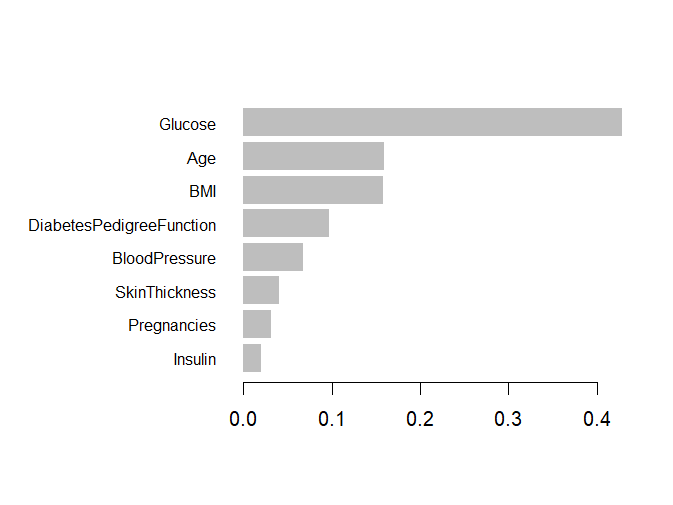
\includegraphics[width=0.80\textwidth]{"C:/Users/msafi/OneDrive/Documents/GitHub/4m_final_project/G1.png"}}
 	\caption{Feature Importance Plot}
 	\label{fig:importance}
\end{figure}

Boosting proved to be an effective method for diabetes classification through achieving an AUC of 0.802 and identifying Glucose, BMI, and Age as the most critical predictors in Figure~\ref{fig:importance}. However, the moderate specificity given by the model (58.21\%) suggests potential overemphasis on predicting positive cases, leading to false positives. Future work could improve model balance through hyperparameter tuning or additional data preprocessing techniques.

\begin{indent}
	
Summarizing the performance results from k-Nearest Neighbours classification, Binary Logistic Regression, Random Forest, and Boosting, we see that each of the models outputted an accuracy of $70.833\%, 76.042\%, 71.88\%$, and $73.44\%$ respectively, indicating that Binary Logistic Regression was the best supervised learning analysis method in predicting the onset of diabetes. 

\end{indent}

\section{Conclusion}
\indent
\onehalfspacing

Throughout this work, we presented various statistical supervised learning analysis methods that could be used to study the \href{https://www.kaggle.com/datasets/hasibur013/diabetes-dataset}{Diabetes Dataset} from \cite{Kaggles}. We effectively showcased the performance accuracy of the k-Nearest Neighbours algorithm, Binary Logistic Regression algorithm, and the ensemble methods: Random Forest and Boosting. Furthermore, the conclusions determined by each of the various methods align with the general scientific consensus on predictors for diabetes in females such as Glucose levels, BMI, Age, and whether an individuals family history has been shown to have a predisposition to diabetes or not. 

Ultimately, although various supervised learning analysis methods have proven to be effective in predicting the onset of diabetes based on several detailed medical diagnostic measurement predictor variables, we remain conscious of challenges associated with some of these methods, such as the large sample size required for logistic regression to output stable results, choosing ‘$k$’ in k-NN through computationally expensive techniques like cross-validation, and the high memory usage and computational cost associated with random forest \citep{7724478}.


 \section{Bibliography}
 \singlespacing
 \bibliographystyle{apa} 
 \bibliography{references}

\end{document}

